\capitulo{4}{Técnicas y herramientas}

Esta parte de la memoria tiene como objetivo presentar las técnicas metodológicas y las herramientas de desarrollo que se han utilizado para llevar a cabo el proyecto.

\section{Herramientas utilizadas}
\begin{itemize}
\tightlist
\item \textbf{Python}: Python es un lenguaje de programación de alto nivel ampliamente utilizado en el campo del aprendizaje automático y la inteligencia artificial. Esto es debido, en parte, a que posee una gran cantidad de bibliotecas y frameworks que facilitan el procesamiento de datos y la implementación de algoritmos de inteligencia artificial.
En este proyecto, Python se ha utilizado para la implementación del back-end. Se han aprovechado su conjunto de bibliotecas para realizar el desarrollo Web (Flask), procesamiento de datos (Librosa, NumPy, Pandas) y métodos de aprendizaje automático (TensorFlow y Scikit-learn).

\item \textbf{librosa}: librosa es una biblioteca de Python utilizada para el análisis y procesamiento de audio. Proporciona de una manera sencilla el acceso a métodos y funciones para realizar análisis, extracción y visualización de características de audio.

\item \textbf{TensorFlow}: TensorFlow es una biblioteca de código abierto utilizada en el campo del aprendizaje automático. Proporciona la posiblidad de implementar redes neuronales complejas de una forma sencilla con grandes volúmenes de datos.

\item \textbf{scikit-learn}: scikit-learn es una biblioteca de aprendizaje automático de Python que proporciona una amplia gama de algoritmos y herramientas para el análisis de datos y la construcción de modelos. Incluye funciones para la división de conjuntos de datos en conjuntos de entrenamiento (\textit{train} y \textit{prueba}) que han sido utilizadas en este proyecto.

\item \textbf{NumPy}: NumPy es una biblioteca de Python utilizada para realizar cálculos numéricos en matrices y matrices multidimensionales. 

\item \textbf{Pandas}: bibliteca de código abierto en Python que proporciona herramientas de análisis de datos.

\item \textbf{Flask}: 
\end{itemize}

\section{Justificación de las herramientas utilizadas}

\subsection{Lenguaje de programación}
\textbf{Lenguajes de programación planteados}: Python, Go, C

\textbf{Lenguajes de programación elegido}: Python

A continuación se presentan algunas justificaciones que han decantado el desarrollo del proyecto en lenguaje Python en comparación con otros lenguajes de programación.

\textbf{Integraciones}: Python cuenta con una completa integración con la mayoría de bibliotecas y frameworks especializados en aprendizaje automático, como TensorFlow, scikit-learn, PyTorch, Keras entre otros. 
En el caso de C, aunque existen algunas bibliotecas como \textit{mlpack}, \textit{libsvm} o una API para controlar TensorFlow (\textit{libtensorflow}) su comunidad de aprendizaje automático es bastante más pequeña que la de Python, por lo que hay menos soporte y recursos disponibles.
En cuanto a Go, su implementación en este proyecto hubiera sido muy interesante debido a ser un lenguaje moderno, rápido y muy popular, pero ocurre lo mismo que con C. Su soporte para aprendizaje automático y procesamiento de datos es pequeña por lo que su suporte y recursos son escasos.
Esto ha sido vital para elegir Python por encima del resto de lenguajes planteados.

\textbf{Rendimiento}: En este apartado los ganadores claros son C y Go, al tratarse de lenguajes compilados, pero en este proyecto el rendimiento bruto no es la prioridad como pueden ser la implementación de algoritmos de aprendizaje automático o el tratamiento de datos.
Por eso mismo se ha elegido Python teniéndo en cuenta que aunque es el que menor rendimiento tiene, es el que otorga un mayor valor al proyecto.

\subsection{Biblioteca de aprendizaje automático}
\textbf{Bibliotecas planteadas}: TensorFlow, Pytorch, Scikit-learn

\textbf{Bibliotecas elegidas}: TensorFlow y Scikit-learn (como herramienta de partición de datos).

\textbf{Integraciones}: tanto TensorFlow, Pytorch como Scikit-learn ofrecen excelentes integraciones con Python. Por lo que este apartado no ha sido importante para valorar la elección entre uno u otro.

\textbf{Enfoque y alcance}: Tanto TensorFlow como Pytorch son bibliotecas de aprendizaje automático de propósito general con soporte para aprendizaje profundo y grandes volumenes de datos. En cambio Scikit-learn es una biblioteca de aprendizaje automático centrada en algoritmos tradicionales y no es adecuado para grandes volúmenes de datos.
Por estas razones se descarta Scikit-learn como una opción viable para entrenar el modelo planteado en este proyecto, aunque se ha utilizado como biblioteca de métodos de procesamiento del conjunto de datos mediante sus herramientas de partición de conjunto de datos (\textit{train\textunderscore test\textunderscore split}).

\textbf{Rendimiento}: tanto TensorFlow como Pytorch poseen soporte para entrenamiento con GPU o TPU, por lo que su rendimiento es muy similar. En este caso la elección ha sido utilizar TensorFlow debido a su mayor documentación y posibilidad de configuración.

\subsection{Framework web}
\textbf{Frameworks web planteados}: Flask, Django

\textbf{Framework web elegido}: Flask

\textbf{Rendimiento}: Flask y Django poseen un rendimiento similar en la mayoría de ocasiones aunque es posible, que en ciertas ocasiones, Flask sea algo más rápido debido a su naturaleza.

\textbf{Enfoque}: Flask sigue una filosofía más simple y minimalista en su desarrollo. Esto ayuda a que su implementación en el proyecto sea más sencilla y \textit{directa}. En cambio Django sigue un patrón de diseño (MVC) más estricto y con muchas funciones que en este proyecto no han sido necesarias.
Por estas razones se ha escogido Flask como la opción para implementar la aplicación web.

\section{Técnicas utilizadas}

Se han utilizado diversas técnicas y metodologías para llevar a cabo el desarrollo y entrenamiento de los modelos de aprendizaje automático.

(En el documento \textit{Anexos} se describe de una forma mucho más profunda el desarrollo metodológico del proyecto.)

\subsection{Procesamiento y extracción de características de audio}

Para el procesamiento y extracción de características de audio, se ha utilizado la biblioteca librosa en Python. Cómo se ha mencionado anteriormente, librosa permite el análisis y procesamiento de audio de una manera sencilla y se ha utilizado para extraer las características de audio para después alimentar al algoritmo de aprendizaje automático.

\subsection{División del conjunto de datos}

Para dividir el conjunto de datos en conjuntos de entrenamiento, prueba y validación, se ha utilizado la biblioteca scikit-learn. 
Scikit-learn proporciona una función llamada \textit{train\textunderscore test\textunderscore split} que permite dividir el conjunto de datos en partes destinadas para el entrenamiento y la evaluación del modelo.
Esta técnica de división del conjunto de datos es fundamental para evaluar la capacidad de \textbf{generalización} del modelo y evitar el \textbf{sobreajuste}.

\begin{figure}
  \centering
  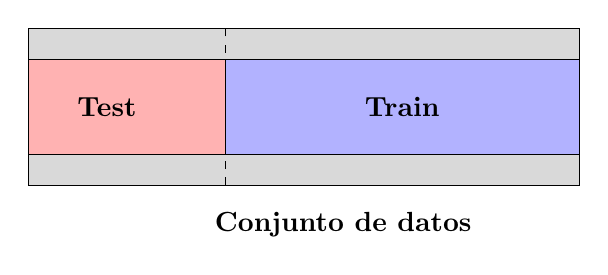
\begin{tikzpicture}
    % Ancho de los conjuntos de entrenamiento y prueba
    \def\datasetwidth{6}
    
    % dataset
    \draw[fill=gray!30] (-1,0) rectangle (\datasetwidth,2);
    
    % test
    \draw[fill=red!30] (-1,0.4) rectangle (1.5,1.6);
    \node at (0,1) {\textbf{Test}};
    
    % train
    \draw[fill=blue!30] (1.5,0.4) rectangle (\datasetwidth,1.6);
    \node at (3.75,1) {\textbf{Train}};
    
    \draw[dashed] (1.5,0) -- (1.5,2);
    
    \draw[dashed] (-1,0.4) -- (\datasetwidth,0.4);
    \draw[dashed] (-1,1.6) -- (\datasetwidth,1.6);
    
    % Etiqueta del conjunto completo
    \node at (\datasetwidth/2,-0.5) {\textbf{Conjunto de datos}};
  \end{tikzpicture}
  \caption{División del conjunto de datos}
\end{figure}

\subsection{Redes neuronales con TensorFlow}

Para realizar el entrenamiento de los datos, se han utilizado redes neuronales implementadas con la biblioteca TensorFlow.

En este proyecto, se han utilizado diferentes arquitecturas de redes neuronales, como redes neuronales convolucionales (CNN) y redes neuronales multicapa. 
Estas arquitecturas son adecuadas para tareas de procesamiento de audio y han demostrado ser efectivas en la clasificación y reconocimiento de patrones en audio.

Las redes neuronales se entrenan actualizando los pesos y los sesgos de la red iterativamente para minimizar la pérdida (\textit{loss}). Una vez entrenadas, las redes neuronales realizan predicciones sobre nuevos datos de audio, clasificándolos en categorías o estilos musicales.